\documentclass[cmfonts]{witpress}
\usepackage{todonotes}
\usepackage{siunitx}
\usepackage{amsmath}
\usepackage{bm}
\usepackage{cleveref}
\usepackage{amssymb}
\usepackage{subcaption}
\captionsetup{compatibility=false}
% \usepackage{natbib}
\bibliographystyle{witpress}


\begin{document}


\title{Improvement of crash forces in structures using optimization tools.}

\author{L. E. Romera, L. Pire, M. Costas, J. Paz, J. D\'iaz, S. Hern\'andez.}

\address{Structural Mechanics Group, Universidade da Coru\~na, Spain.}

\maketitle

\begin{abstract}
This work describes an investigation on the structural optimization of the crash response of aircraft or road vehicle crash boxes, where the force pulse due to frontal impact or hard landing wanted to be kept as stable as possible while reducing the mass of the energy absorbing systems. The objective functions were minimized in a multi-objective approach using metamodeling on FE models and genetic evolutionary algorithms. Finite element models were subjected to a frontal impact test against a simplified rigid wall in the case of the car model, or to hardlanding impact for the fuselage model. Force-time curves was obtained from the analysis and suitably filtered. The objective functions were calculated as the variance of this force-time curves and the total structural mass. The objective was to obtain a force-time curve which was as close as possible to the ideal dissipator curve, with lower values of the peaks of acceleration experienced by the occupants; and to minimize the mass for fuel saving and environmental reasons. To that end, optimization strategies were planned carefully to deal with problems which are typical in crashworthiness optimization like expensive computation times and numerical noise.
\end{abstract}\\
\emph{Keywords: crashworthiness, injuries reduction, size optimization, surrogate models.}

\section{Introduction}
Occupant safety is a key issue on vehicle and aircraft design nowadays, and crashworthy elements are required to absorb the energy during a crash and minimize the effects on the occupants. Aircraft and vehicles are nowadays provided with crash boxes to absorb the impact energy through deformation in order to protect the passengers. They are usually tube-shaped and made of several parts that require some kind of bonding.

On the other hand, structural adhesives have improved their mechanical properties in recent years and can be now used with confidence in heavy duty applications. Interest on them is also raising up in scientific fields thanks to these enhancements and to the recent development of validated numerical models.
\begin{figure}[htpb]
	\centering
	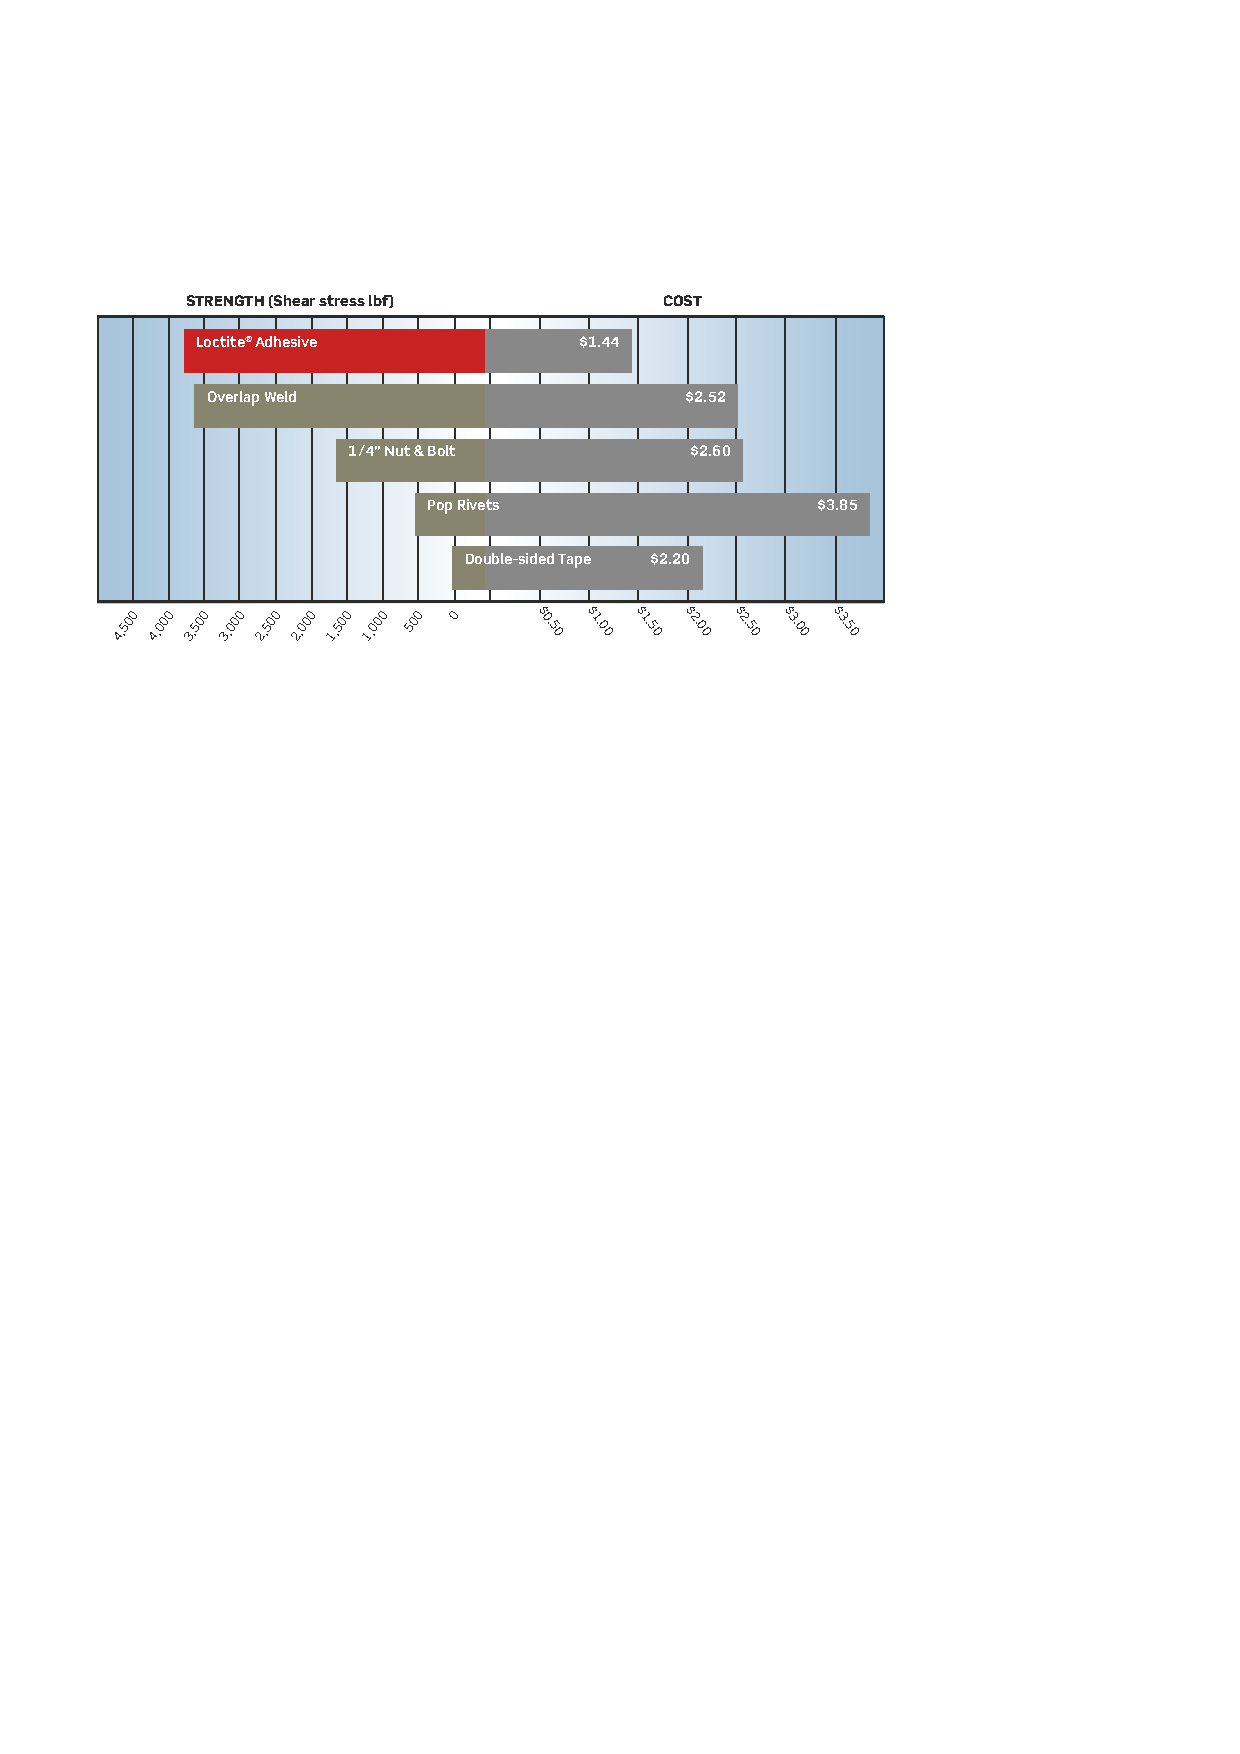
\includegraphics[width=\linewidth]{./figures/IMG_CUTRES/comparison}
	\caption[Qualitative strength and cost comparison of different joining solutions.]{Qualitative strength and cost comparison of different joining solutions. Taken from \cite{superyacht}.}
	\label{fig:comparison}
\end{figure}

As shown in \Cref{fig:comparison}, adhesives are very competitive both in bonding strength and in economical manufacturing costs \cite{superyacht}. In order to check adhesive's suitability for their use in crashworthy elements, this research develops numerical models of adhesively bonded crash boxes subjected to impact loads using finite element models. Information and data present in the literature are used to create and validate these models in order to ensure the accuracy of the results.

\section{Finite element model}
The modeled crash box consists of two adherend cold-formed sheets made of steel that create a tube of square section bonded together with an epoxy adhesive. The joint is practiced on the surface of two flanges on each adherend side. In order to ease the model validation, the crash box geometry was created to reflect those tested by \cite{Peroni2009} and later modeled by \cite{Scattina2011}. In particular, the two sections depicted in \cref{fig:crash_box} are modeled in the present study.
\begin{figure}[ht]
  \centering
  \begin{minipage}[b]{.48\linewidth}
    \centering
    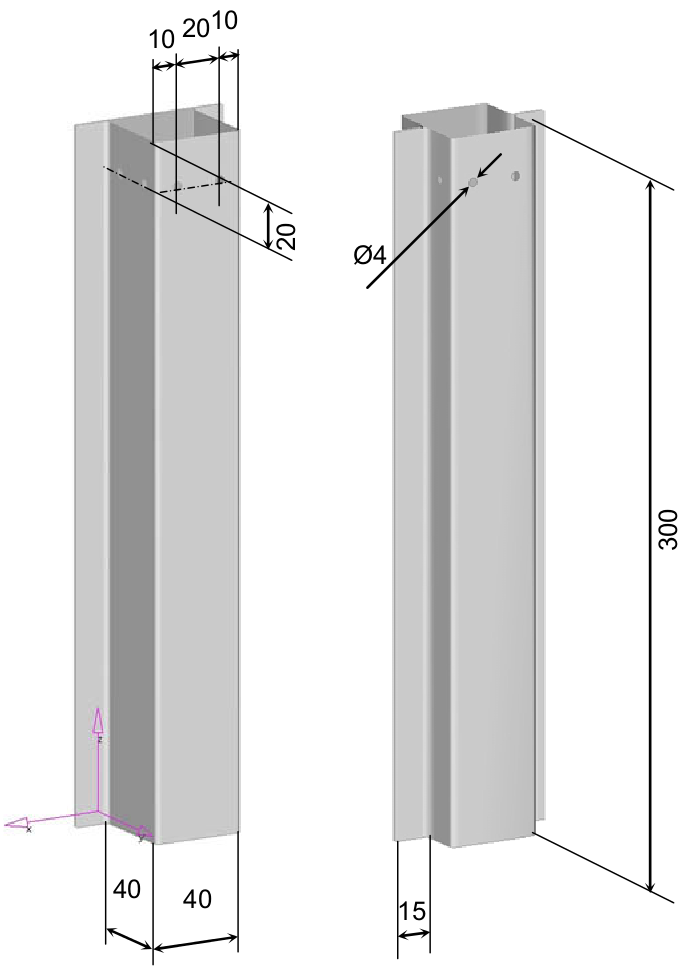
\includegraphics[width=\linewidth]{figures/IMG_CUTRES/medidas_cb}
    \subcaption{Dimensions of the modeled crash boxes, in millimeters. Taken from \cite{Peroni2009}.}
    \label{fig:crash_box}
  \end{minipage}
  \hfill
  \begin{minipage}[b]{.48\linewidth}
    \centering
    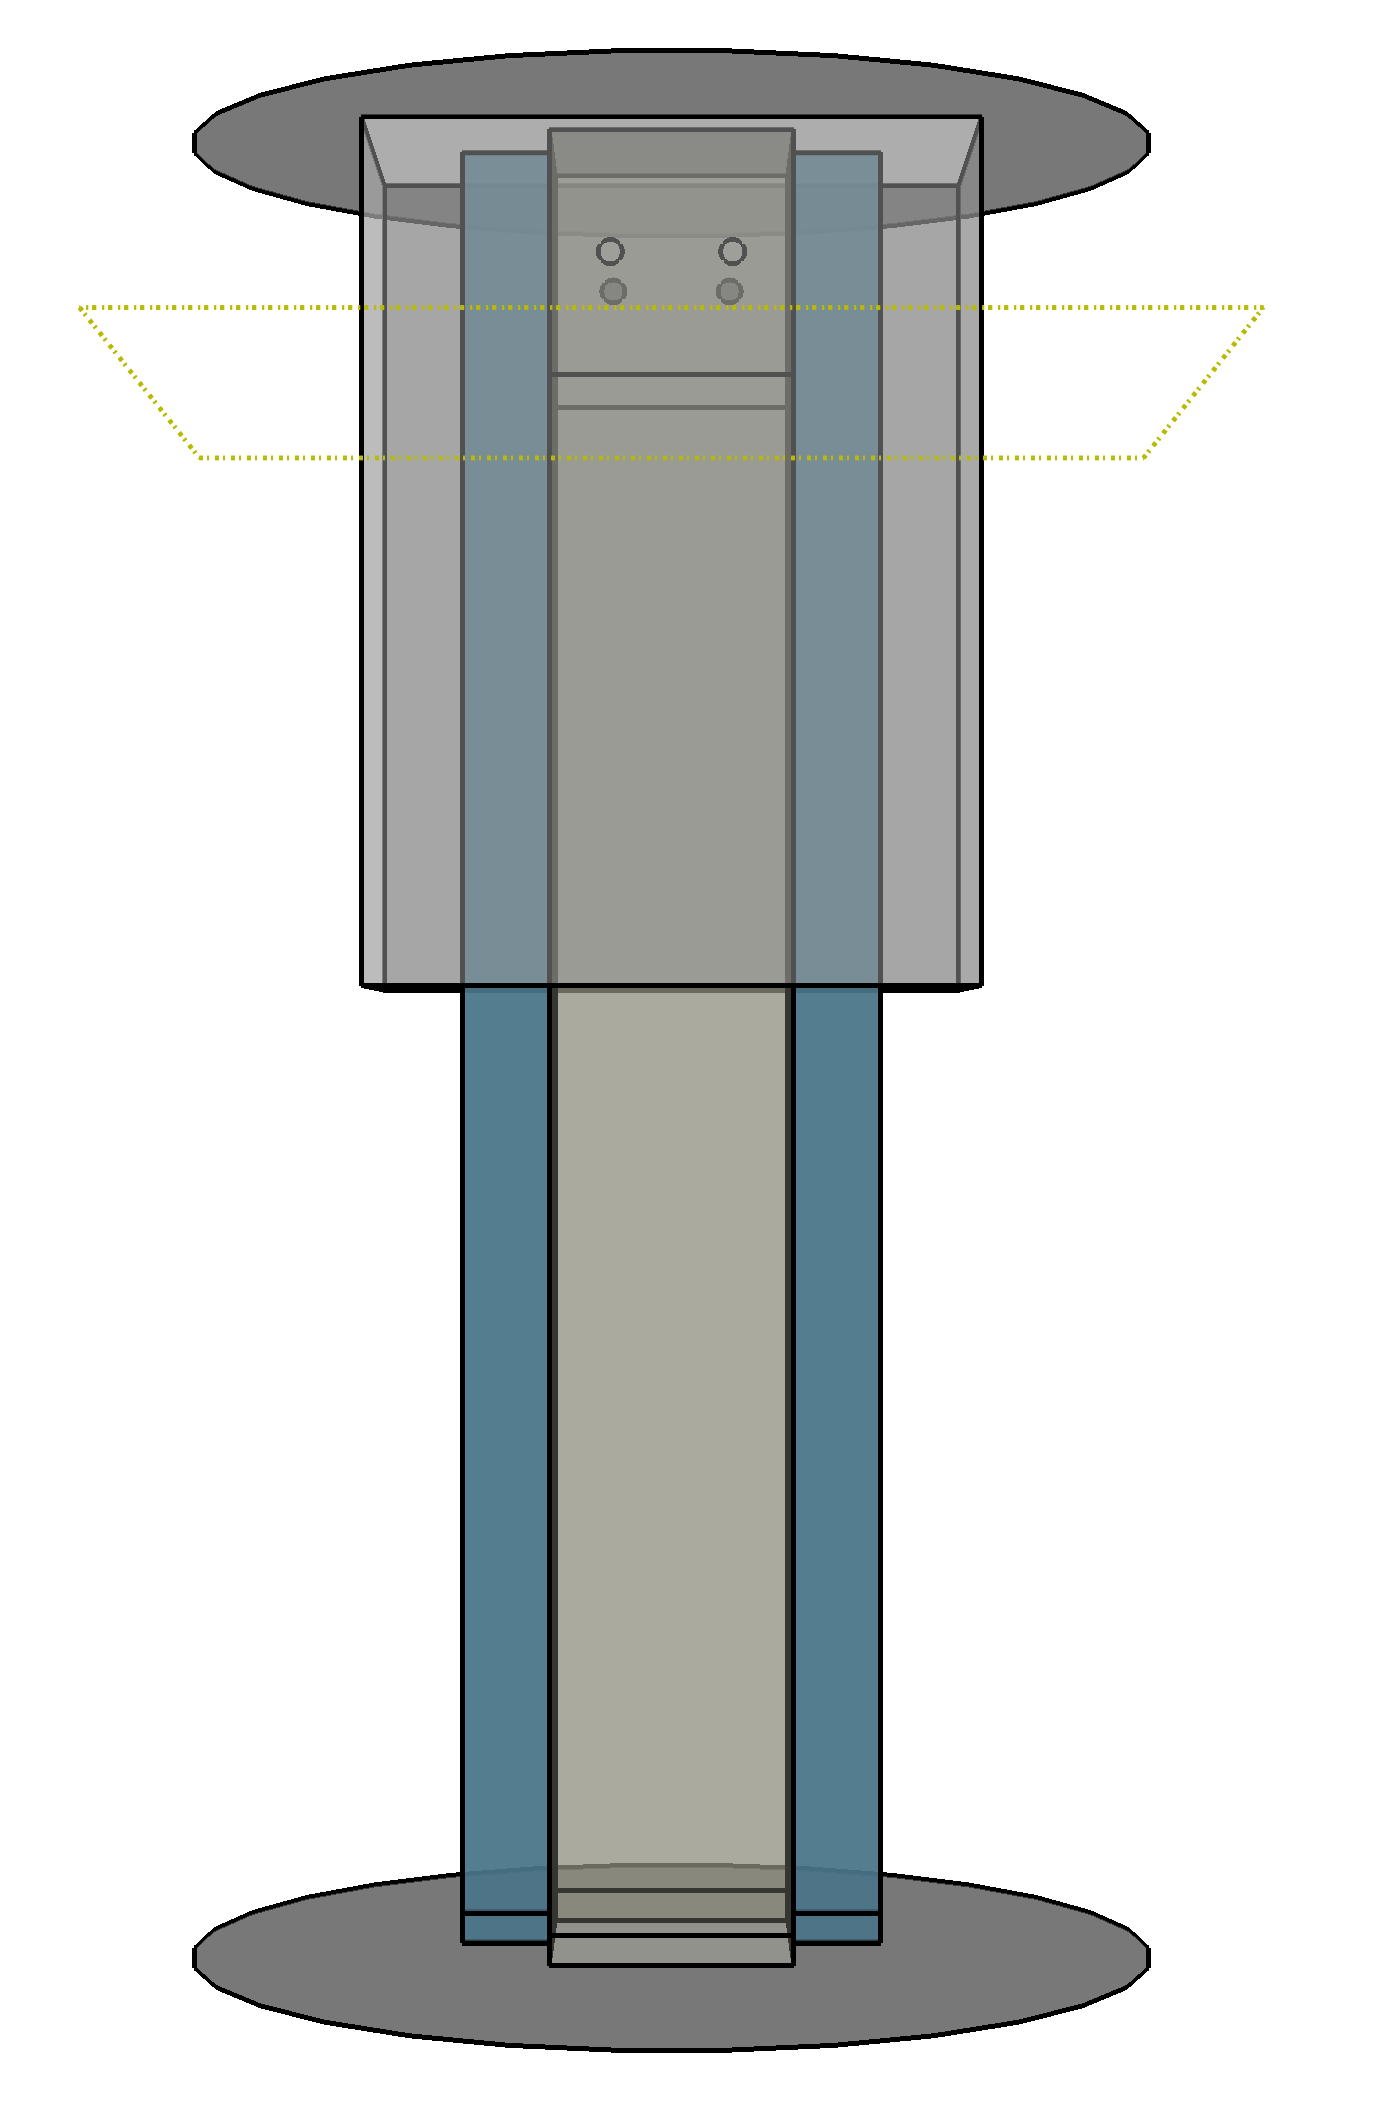
\includegraphics[width=0.9\linewidth]{figures/IMG_CUTRES/general_transp}
    \subcaption{General view of the model with the bounding box.}
    \label{fig:general}
  \end{minipage}
  \caption{Dimensions of the studied crash boxes and view of the finite element model including a bounding box.}
  \label{fig:modelo}
\end{figure}

The tube is crushed between two rigid plates, one fixed and the other moving at impact speed (see \Cref{fig:general}). In order to ease the formation of a stable collapse mechanism, a triggering is machined near the front end of the tube. The trigger starts a desired collapse mode in that area. Due to the high slenderness of the tube, difficulties were found in order to achieve stable collapse mechanisms. On their place, tubes diverted from their axis. Trying to avoid these critical situations, four rigid plates on a rectangular section around the crash tube were added to the model as a bounding box. Its section was $\num{100}\times\SI{60}{\mm}$ and co-centered with the crash box.

The impact plate moved during the simulation at $\SI{10}{\m/\s}$ on a total distance equal to half of the total tube's length, resulting in a total analysis time of $\SI{0.015}{\s}$. Rotational degrees of freedom were fixed on the frontal plate. The rear plate had all degrees of freedom restrained.

The last $\SI{5}{\mm}$ of the crash tube had all degrees of freedom fixed (see \cref{fig:general}), except displacement on the impact direction in order to allow the reaction force measurement commented before. This way, numerical issues due to excesive unrestrained degrees of freedom on the whole tube were prevented.

Peeling problems were found near the impact head end during the development of the study. \cite{Peroni2009} solved this situation by adding two rivets on the bonded flanges at the triggered section in order to avoid excesive debonding on that part of the tube in the initial phases of the impact and, thus, prevent critical situations. In this study, this was simulated by a $\SI{2}{\mm}$-diameter spot-weld at the same location.

\subsection{Materials}

The model is made up of two different materials: the adherends of the tube are made of steel and the adhesive is the epoxy-based, heat-cured Loctite Hysol 9514.

According to \cite{manufCatalog}, the shear strength of the adhesive is $\SI{44}{\MPa}$, although this parameter is subject to variation depending both in cure temperature and time. The bulk modulus is $\SI{1460}{\MPa}$ and the adhesive's density is $\SI{1.30}{\tonne/\m^3}$ \cite{manufCatalog}. The constitutive behavior was supposed to be isotropic linear elastic \cite{SernaMoreno2015} up to failure start. An uncoupled traction elastic behavior \cite{Sadowski2010, Sadowski2011, Scattina2011, Sadowski2014} on 3D cohesive finite elements was chosen.

\cite{Scattina2011} obtained adhesive stiffnesses through the inverse method, which are summarized in \cref{tab:ads_params}. These same parameters were used in the present study, as their results could be validated with the model.
\begin{table}
	\centering
	\begin{tabular}{llrl}
	\hline
		Parameter & Description & Value & \\
		\hline
		$E_{N}$ & Stiffness in normal direction & $\num{5e9}$ & $\si{\kN/\m^2}$ \\
		$E_{T}$ & Stiffness in an in-plane direction & $\num{8e7}$ & $\si{\kN/\m^2}$ \\
		$G_{Ic}$ & Energy release rate for mode I & $\num{2028}$ & $\si{\J/\m^2}$ \\
		$G_{IIc}$ & Energy release rate for mode II & $\num{11853}$ & $\si{\J/\m^2}$ \\
		$\sigma_{n}^{0}$ & Peak traction in normal direction & $\num{130}$ & $\si{\MPa}$ \\
		$\tau_{II}^{0}$ & Peak traction in tangential direction & $\num{42.5}$ & $\si{\MPa}$ \\
		\hline
	\end{tabular}
	\caption[Loctite Hysol 9514 parameters.]{Loctite Hysol 9514 parameters. Taken from \cite{Scattina2011}.}
	\label{tab:ads_params}
\end{table}

Contact failure modeling ---corresponding to adhesive failure--- resulted in some simulation problems, so adhesives and adherends were kept together with a simplified tie constraint. Thus, failure definitions were only included in the bulk material, obviating the contact/adhesive failure as suggested by several authors \cite{Greve2007, Loureiro2010, Sadowski2010, Sadowski2011, Scattina2011, Sadowski2014, SernaMoreno2015}, although the modeled cohesive damage parameters include the effect of both adhesive and cohesive resistance.

Regarding the metal sheets, in order to make the model comparable to the experiments carried out by \cite{Peroni2009}, steel was chosen for these adherends. In the present study, it is defined as an isotropic elastic-plastic material, with a density of $\SI{7.85}{\tonne/\m^3}$.

The elastic part of the adherend stress-strain curve is defined as linear, with an elastic modulus of $\SI{200}{\GPa}$ and a Poisson ratio of $\num{0.3}$. An initial yield stress of $\SI{190}{\MPa}$ is set, and work hardening is defined through a tangent plastic modulus of $\SI{950}{\MPa}$ \cite{Peroni2009}.



\subsection{Finite element mesh and simulation setup}

The use of cohesive elements allowed to make the adhesive's mesh much coarser due to their aspect ratios requirements. These elements were created with a size of $\SI{2.0}{\mm}$, and had only one element in the $\SI{0.3}{\mm}$ layer thickness. Other tested element types, specifically solids, had problems if side lengths were bigger than about $\SI{0.5}{\mm}$, and were completely unfeasible with lengths larger than $\SI{1.0}{\mm}$ approximately.

% Tie (include image)
The tie constraint included in Abaqus enabled non-coherent meshes between adhesive and adherend (\cref{fig:mesh_detail_coh3d_comparison}). This way, finer meshes could be implemented on the adhesive in order to improve the representation of the failure progression without increasing the adherend element recount by leaving a coarser mesh there.
\begin{figure}[htpb]
	\centering
	\begin{minipage}[b]{.7\linewidth}
		\centering
		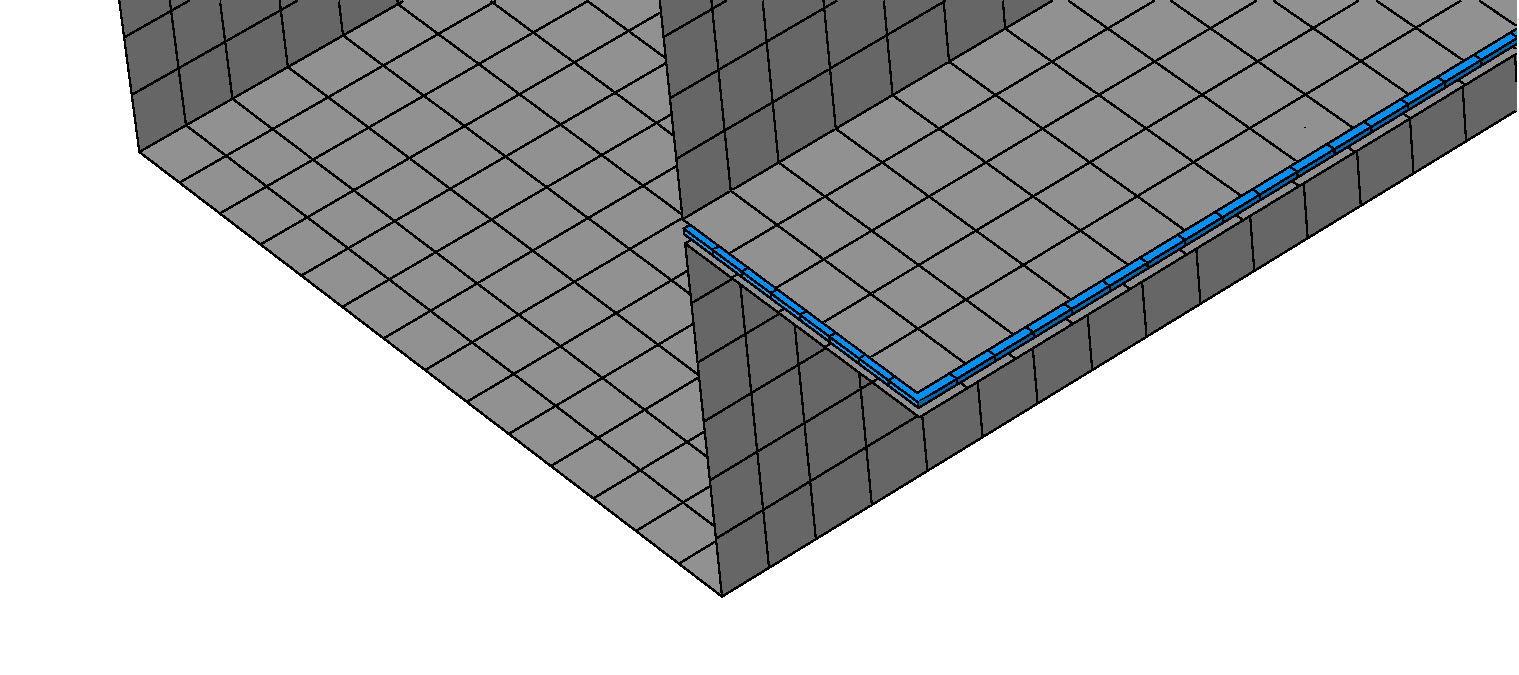
\includegraphics[width=0.7\linewidth]{figures/IMG_CUTRES/mesh_detail_coh3d_comparison}
		\caption[Detail of COH3D mesh on the adhesive layer.]{Detail of COH3D mesh on the adhesive layer (blue).}
		\label{fig:mesh_detail_coh3d_comparison}
	\end{minipage}
	\\[10pt]
	\begin{minipage}[b]{.7\linewidth}
		\centering
		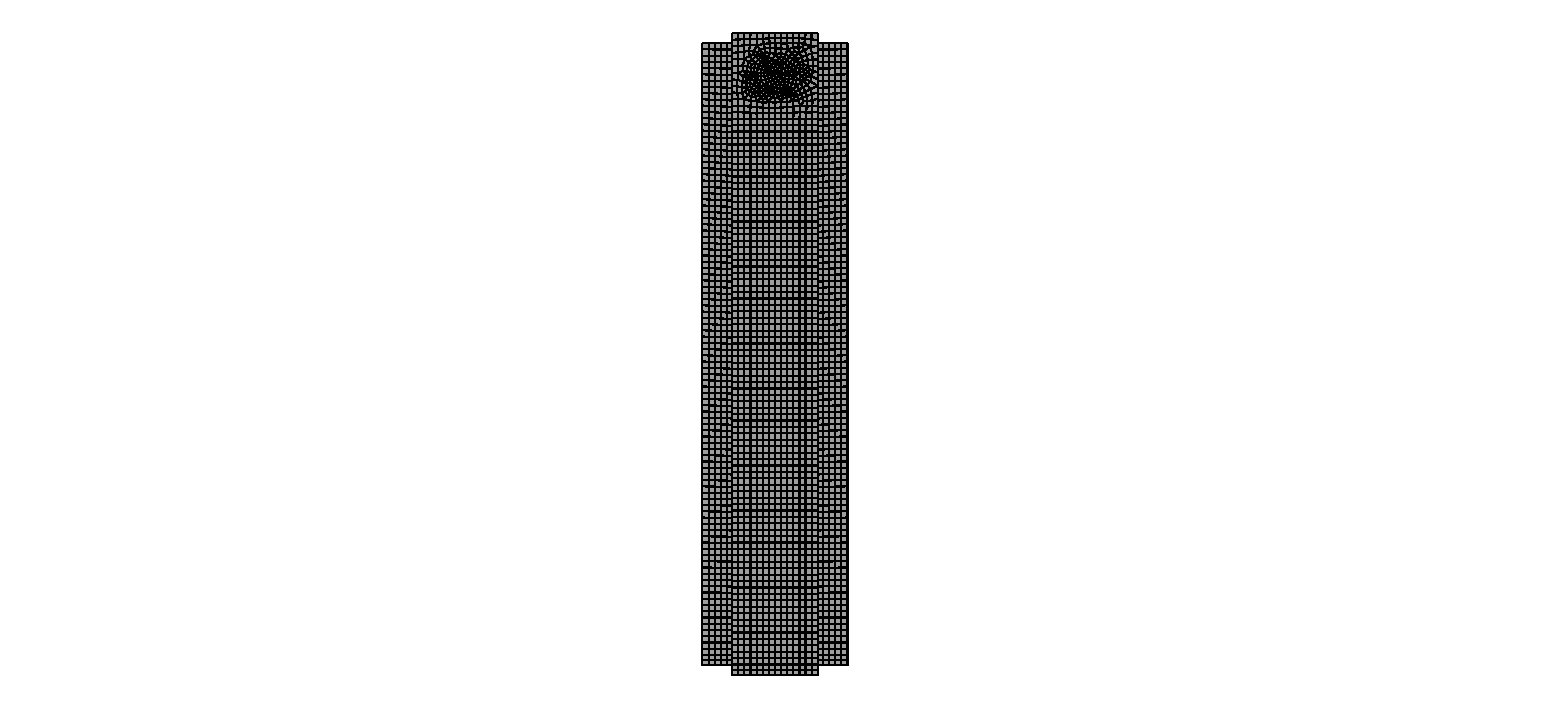
\includegraphics[width=\linewidth]{figures/IMG_CUTRES/mesh}
		\caption{General mesh of the crash box.}
		\label{fig:mesh}
	\end{minipage}
	\caption{Views of the mesh of the finite element model: globral view and detail view of the adhesive.}
	\label{fig:mallas}
\end{figure}


The finite element package Abaqus Explicit is used in this research, on is version 6.13 \cite{Abaqus613Manual} running on a high performance computing cluster. Jobs running on loop parallelization over $16$ cores took about $\SI{8}{\hour}$ to finish. Domain parallelization turned out to be inefficient in this case due to poor network performance.

\subsection{Simulation results}


In order to filter high frequency effects, a SAE 600 filter was applied to the simulation results \cite{Huang}. \Cref{fig:F-D_rough} provides the obtained force-displacement curves and the results obtained in \cite{Peroni2009}. In this figure the nomenclature is as follows:
\begin{itemize}
	\item ``AR'' or ``BR'' indicating the cross-section of the tube: ``A'' for the top-hat, and ``B'' for the double hat.
	\item An ``R'' after the underline indicates that the crash box had riveting in the triggered cross section.
	\item ``Sb'' after the underline marks the presence of a stabilizing box in the model.
\end{itemize}

\begin{figure}[htpb]
	\centering
	\begin{minipage}[b]{.7\linewidth}
		\centering
		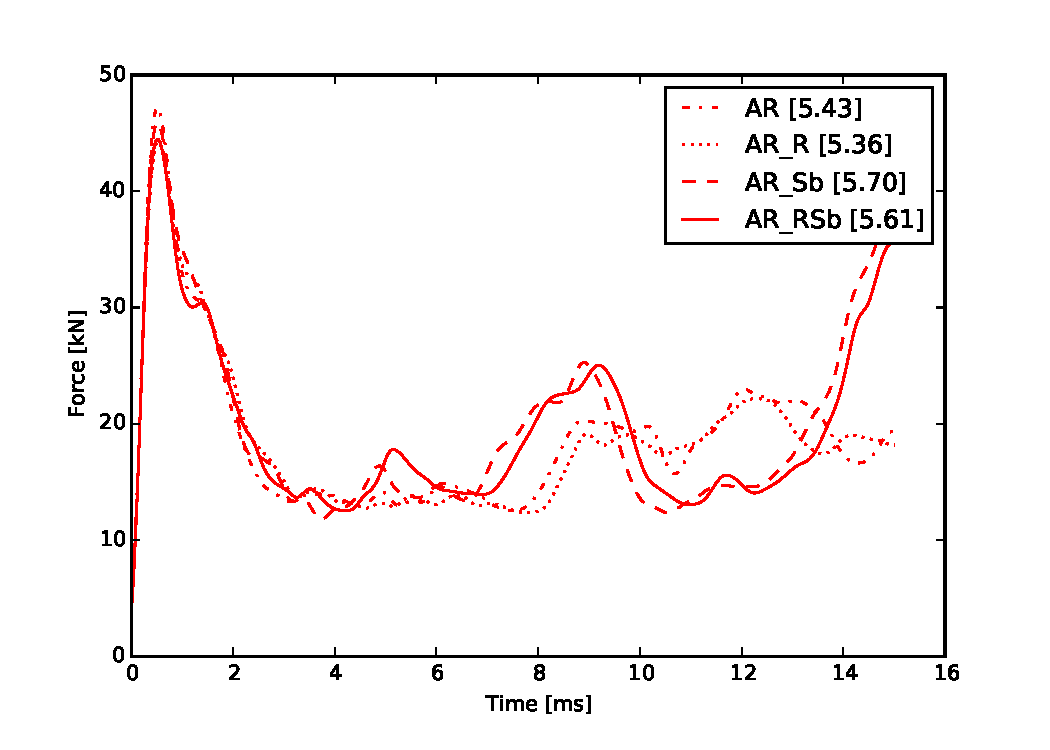
\includegraphics[width=\linewidth]{IMG_CUTRES/AR}
	\end{minipage}
	\quad
	\begin{minipage}[b]{.7\linewidth}
		\centering
		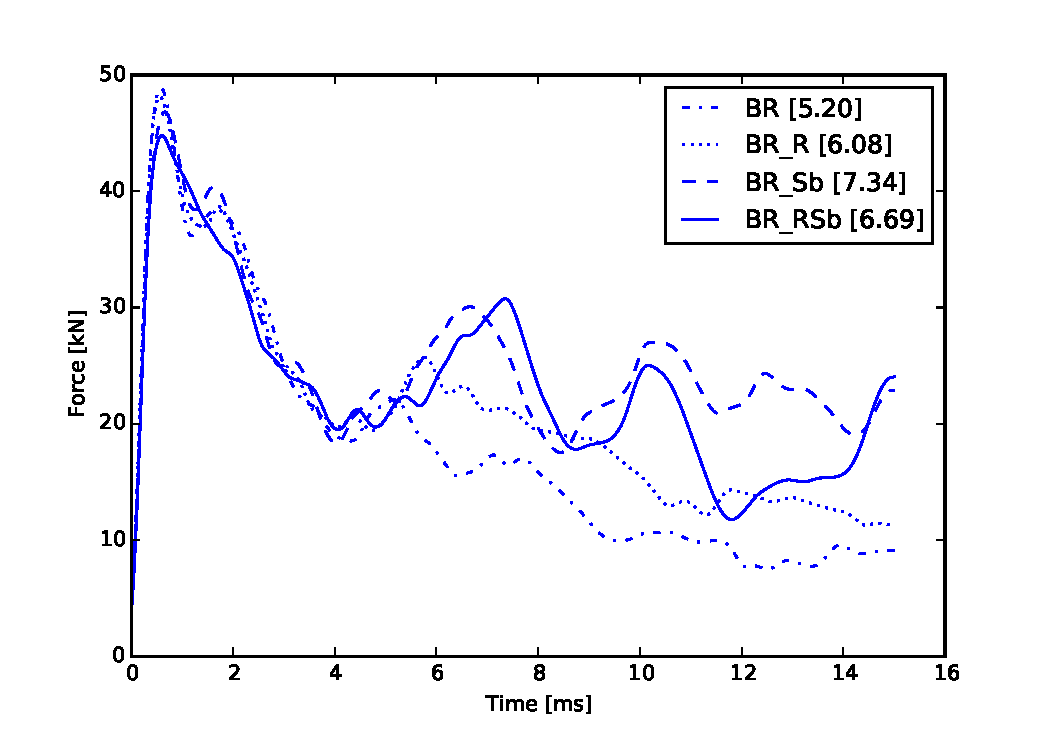
\includegraphics[width=\linewidth]{IMG_CUTRES/BR}
	\end{minipage}
	\quad
	\begin{minipage}[b]{.7\linewidth}
		\centering
		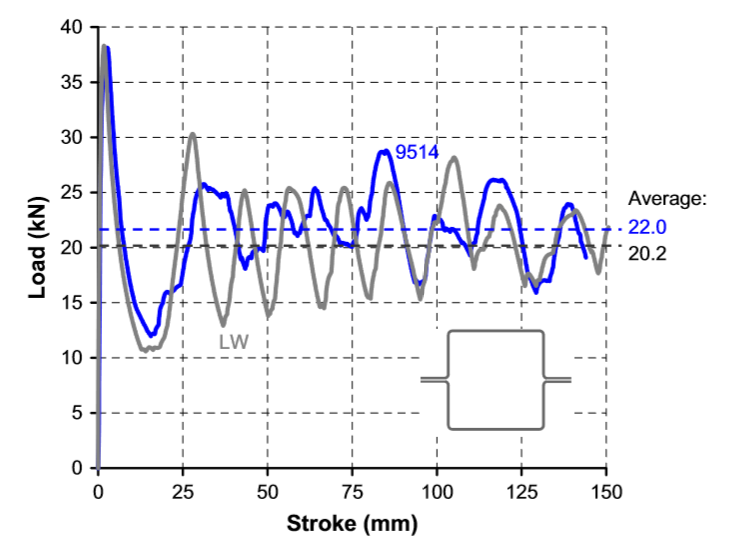
\includegraphics[width=\linewidth]{peroni_qstat_fd}
	\end{minipage}	
	\caption[Force-displacement curves for top-hat and double hat sections with different modeled configurations.]{Force-displacement curves for top-hat and double hat sections with different modeled configurations and curves in \cite{Peroni2009}. Specific energy absorption is provided in brackets in $\si{\kJ/\kg}$.}
	\label{fig:F-D_rough}
\end{figure}

Qualitatively, this curves are very similar to those obtained by \cite{Peroni2009}. \Cref{fig:F-D_rough} depicts also a quasi-static test performed by these authors with the same section and bonding solution. Facing these similitudes, the model is considered valid. A view of the progressive collapse of the top-hat section is provided in \Cref{fig:stable}

In general, a uniform force-displacement curve would be the most desirable scenario, as it would imply maximizing the $E_\text{a}$  with the minimum $P_\text{peak}$. Thus, the best solution will be the one with the most constant response.

\begin{figure}
	\centering
	\begin{minipage}[b]{.15\linewidth}
		\centering
		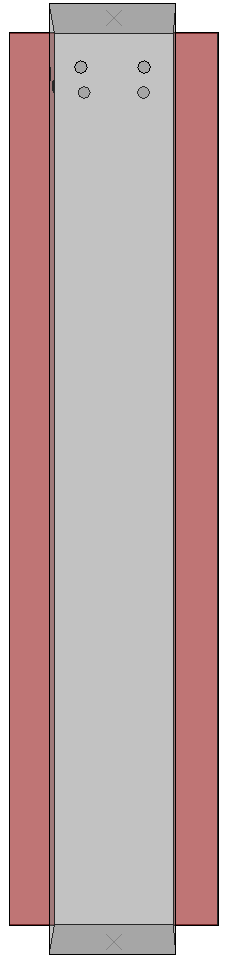
\includegraphics[width=\linewidth]{IMG_CUTRES/a0}
	\end{minipage}
	\hfill
	\begin{minipage}[b]{.15\linewidth}
		\centering
		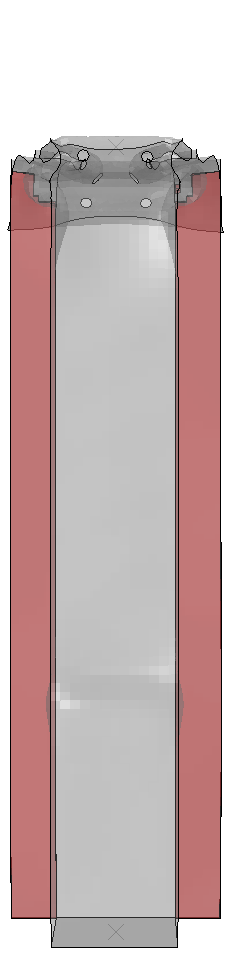
\includegraphics[width=\linewidth]{IMG_CUTRES/a3}
	\end{minipage}
	\hfill
	\begin{minipage}[b]{.15\linewidth}
		\centering
		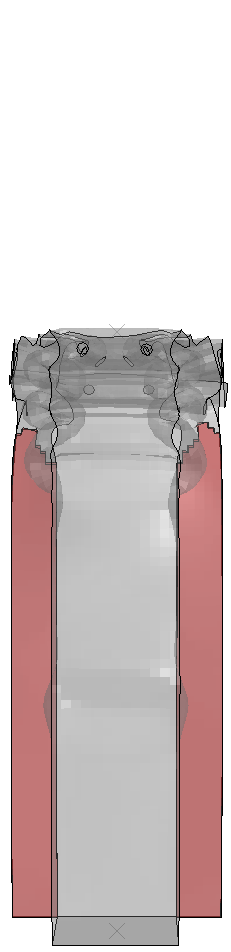
\includegraphics[width=\linewidth]{IMG_CUTRES/a7}
	\end{minipage}
	\hfill
	\begin{minipage}[b]{.15\linewidth}
		\centering
		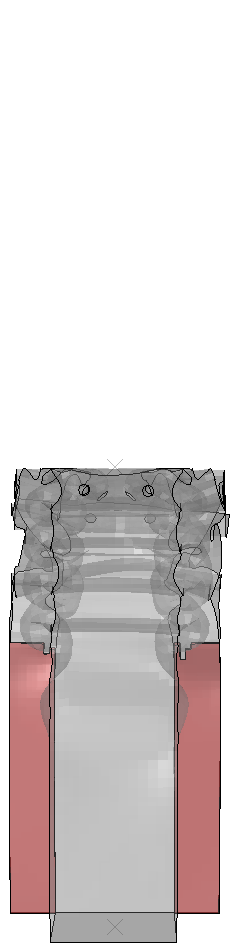
\includegraphics[width=\linewidth]{IMG_CUTRES/a10}
	\end{minipage}
	\caption[Stable collapse mechanism achieved in the top-hat tube with bounding box.]{Stable collapse mechanism achieved in the top-hat tube with bounding box (hidden). Semi-transparent projection with adhesive in red.}
	\label{fig:stable}
\end{figure}


\section{Optimization strategy}

\subsection{Surrogate-based methods}

In order to optimize the specimen, a surrogate-optimization approach is used. Therefore, the computationally-expensive  objective functions of the model are replaced by another functions less costly to evaluate. 

Firstly, with the parametrized model, a sampling of $n$ samples is performed, relying on the LHS technique. This method creates a set of data with homogeneous projections on each variable axis, so that no superimposed projections appear. 

Once the sampling is obtained, the surrogate model is created. The Multivariate adaptive regression splines (MARS) method is chosen, where the surrogate functions are adjusted with cubic splines following the next expression
\begin{equation}\label{eq:mars}
\hat{f}\left ( \bm{x} \right )= \sum_{m=1}^{M}a_{m}B_{m}\left ( \bm{x} \right ),
\end{equation}
where $B_{m}$ are the power basis functions, $a_{m}$ the coefficients of the functions, and $M$ is the number of functions. This method is more thoroughly explained in \cite{Friedman1995197}. 


With the surrogate-based model created, multi-objective optimization is performed. Traditional methods involving gradient-based and Hessian-based information are not very useful for these surrogate models, since many local minima are found in the function, yielding only misleading results. Therefore, evolutionary algorithms are used, since this type of methods are slower but dodge local minima with ease. The results are conformed by a Pareto front, corresponding to a range of results. This Pareto front points cannot improve the value of one objective function without worsening the value of at least one other objective function. \Cref{fig:Pareto} shows an example of a Pareto front opposing the energy absorbed by the specimen and its mass, where the line constitutes the set of optima for these metrics.

\begin{figure}[htpb]
  \centering
   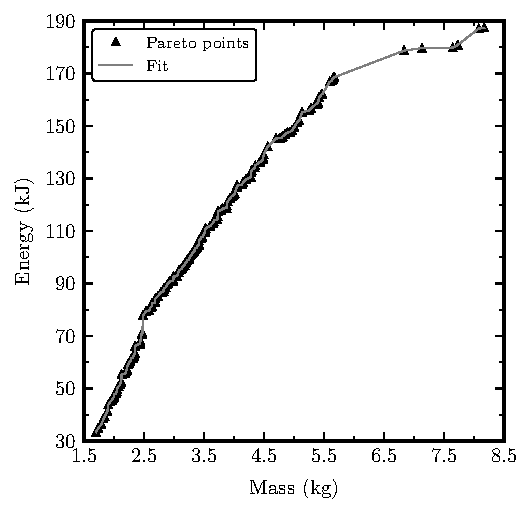
\includegraphics[width=.8\columnwidth]{figures/IMG/Pareto}
  \caption{Pareto frontier opposing energy absorbed and mass of the specimen.}
  \label{fig:Pareto}
\end{figure}

% The methods selected for both the single- and the multi-objective optimization are the genetic algorithms from the JEGA Library, developed by \cite{JEGA}, which perform optimization supporting general constraints as well as mixtures of real and discrete variables.

\subsection{Metrics}

The objective functions considered in this research are the absorbed energy ($E_a$), the mass of the specimen ($m$) and the peak load ($P_{peak}$). The mass of the specimen is obtained from the finite element model, and $E_a$ and $P_{peak}$ are obtained from the resulting force-displacement curves.

The force-displacement curve obtained is filtered with a standard SAE 600 filter \cite{J211} before making any calculations, as this removes the high-frequency noise from the curve with a cutoff frequency of ${1000}$ Hz. After this, $E_a$ and $P_{peak}$ are obtained.
% \begin{equation}\label{Ea}
%   E_{a}=\int _{0}^{\delta }F\! \left( z \right) \,dz\,,
% \end{equation}
% where $\delta$ is the total axial crushing distance and $F\! \left( z \right)$ the crushing force at a distance $z$.

% The peak load $P_{peak}$ is defined as
% \begin{equation}\label{Peak}
%  P_{peak}=max\left\{ F\! \left( z \right)  \forall z \in [0,\delta] \right\}
% \end{equation}

The first reason for choosing these metrics is the nature of the design and its aim to improve the crashworthiness of vehicles. The $E_a$ can be easily improved by increasing the thicknesses of the materials, but this would the mass of the specimen and $P_{peak}$. Increasing the mass also  increases the vehicle's fuel consumption and reduces its efficiency; whereas an increase in the $P_{peak}$ means a higher force and acceleration suffered by the passengers of the vehicle, raising the odds of resulting in a serious injury.

Furthermore, other researchers have traditionally optimized the specific energy absorption (SEA) and the load ratio (LR) \cite{Hou2007555}. Thus, they are also evaluated as objective functions, but considering their more complicated comportment and a noisier nature for this model. 

\subsection{Optimization process}

In order to optimize the model, the process is divided into two different stages. Firstly, a parameter study is performed. A simple sampling of the work space for each variable is carried out. With this, a general idea of the variables' behavior is obtained.

% Secondly, single-objective optimization is run for the SEA objective function. Whereas an optimization of the mass and the absorbed energy would provide better results, this can be easier optimized, since the other option requires multi-objective optimization. Both unconstrained and constrained optimization procedures are considered, setting a limit for the peak load constraint in the latter.


Afterwards, multi-objective unconstrained optimization is sought. All objective functions are minimized, and the points obtained as solution cannot be improved in a variable without harming, at least, another one. This last step is the most complete, giving more information of the behavior of the functions and the optimization process, but due to the greater complexity in the evaluation it is computed the last.

\section{Conclusions}
From this research the following conclusions can be drawn:
\begin{itemize}
	\item The crash behavior of adhesively bonded steel crash boxes have been successfully simulated in a commercial finite element package. Results have been validated with experimental data in the literature.
	\item A description of a suitable optimization method for the analyzed crash boxes is provided. A multiobjective algorithm enables the balancing of contrasting objective functions like the specific energy absorption and the peak loads of the structures.
\end{itemize}

\section{Acknowledgments}
The research leading to these results has received funding from the Spanish Government (Ministerio de Economía y Competitividad) under grant agreement DPI2013-41893-R. The authors fully acknowledge the support received.

\bibliography{./references/references}

\end{document}
